% Options for packages loaded elsewhere
\PassOptionsToPackage{unicode}{hyperref}
\PassOptionsToPackage{hyphens}{url}
%
\documentclass[
]{article}
\usepackage{amsmath,amssymb}
\usepackage{lmodern}
\usepackage{iftex}
\ifPDFTeX
  \usepackage[T1]{fontenc}
  \usepackage[utf8]{inputenc}
  \usepackage{textcomp} % provide euro and other symbols
\else % if luatex or xetex
  \usepackage{unicode-math}
  \defaultfontfeatures{Scale=MatchLowercase}
  \defaultfontfeatures[\rmfamily]{Ligatures=TeX,Scale=1}
\fi
% Use upquote if available, for straight quotes in verbatim environments
\IfFileExists{upquote.sty}{\usepackage{upquote}}{}
\IfFileExists{microtype.sty}{% use microtype if available
  \usepackage[]{microtype}
  \UseMicrotypeSet[protrusion]{basicmath} % disable protrusion for tt fonts
}{}
\makeatletter
\@ifundefined{KOMAClassName}{% if non-KOMA class
  \IfFileExists{parskip.sty}{%
    \usepackage{parskip}
  }{% else
    \setlength{\parindent}{0pt}
    \setlength{\parskip}{6pt plus 2pt minus 1pt}}
}{% if KOMA class
  \KOMAoptions{parskip=half}}
\makeatother
\usepackage{xcolor}
\usepackage[margin=1in]{geometry}
\usepackage{color}
\usepackage{fancyvrb}
\newcommand{\VerbBar}{|}
\newcommand{\VERB}{\Verb[commandchars=\\\{\}]}
\DefineVerbatimEnvironment{Highlighting}{Verbatim}{commandchars=\\\{\}}
% Add ',fontsize=\small' for more characters per line
\usepackage{framed}
\definecolor{shadecolor}{RGB}{248,248,248}
\newenvironment{Shaded}{\begin{snugshade}}{\end{snugshade}}
\newcommand{\AlertTok}[1]{\textcolor[rgb]{0.94,0.16,0.16}{#1}}
\newcommand{\AnnotationTok}[1]{\textcolor[rgb]{0.56,0.35,0.01}{\textbf{\textit{#1}}}}
\newcommand{\AttributeTok}[1]{\textcolor[rgb]{0.77,0.63,0.00}{#1}}
\newcommand{\BaseNTok}[1]{\textcolor[rgb]{0.00,0.00,0.81}{#1}}
\newcommand{\BuiltInTok}[1]{#1}
\newcommand{\CharTok}[1]{\textcolor[rgb]{0.31,0.60,0.02}{#1}}
\newcommand{\CommentTok}[1]{\textcolor[rgb]{0.56,0.35,0.01}{\textit{#1}}}
\newcommand{\CommentVarTok}[1]{\textcolor[rgb]{0.56,0.35,0.01}{\textbf{\textit{#1}}}}
\newcommand{\ConstantTok}[1]{\textcolor[rgb]{0.00,0.00,0.00}{#1}}
\newcommand{\ControlFlowTok}[1]{\textcolor[rgb]{0.13,0.29,0.53}{\textbf{#1}}}
\newcommand{\DataTypeTok}[1]{\textcolor[rgb]{0.13,0.29,0.53}{#1}}
\newcommand{\DecValTok}[1]{\textcolor[rgb]{0.00,0.00,0.81}{#1}}
\newcommand{\DocumentationTok}[1]{\textcolor[rgb]{0.56,0.35,0.01}{\textbf{\textit{#1}}}}
\newcommand{\ErrorTok}[1]{\textcolor[rgb]{0.64,0.00,0.00}{\textbf{#1}}}
\newcommand{\ExtensionTok}[1]{#1}
\newcommand{\FloatTok}[1]{\textcolor[rgb]{0.00,0.00,0.81}{#1}}
\newcommand{\FunctionTok}[1]{\textcolor[rgb]{0.00,0.00,0.00}{#1}}
\newcommand{\ImportTok}[1]{#1}
\newcommand{\InformationTok}[1]{\textcolor[rgb]{0.56,0.35,0.01}{\textbf{\textit{#1}}}}
\newcommand{\KeywordTok}[1]{\textcolor[rgb]{0.13,0.29,0.53}{\textbf{#1}}}
\newcommand{\NormalTok}[1]{#1}
\newcommand{\OperatorTok}[1]{\textcolor[rgb]{0.81,0.36,0.00}{\textbf{#1}}}
\newcommand{\OtherTok}[1]{\textcolor[rgb]{0.56,0.35,0.01}{#1}}
\newcommand{\PreprocessorTok}[1]{\textcolor[rgb]{0.56,0.35,0.01}{\textit{#1}}}
\newcommand{\RegionMarkerTok}[1]{#1}
\newcommand{\SpecialCharTok}[1]{\textcolor[rgb]{0.00,0.00,0.00}{#1}}
\newcommand{\SpecialStringTok}[1]{\textcolor[rgb]{0.31,0.60,0.02}{#1}}
\newcommand{\StringTok}[1]{\textcolor[rgb]{0.31,0.60,0.02}{#1}}
\newcommand{\VariableTok}[1]{\textcolor[rgb]{0.00,0.00,0.00}{#1}}
\newcommand{\VerbatimStringTok}[1]{\textcolor[rgb]{0.31,0.60,0.02}{#1}}
\newcommand{\WarningTok}[1]{\textcolor[rgb]{0.56,0.35,0.01}{\textbf{\textit{#1}}}}
\usepackage{graphicx}
\makeatletter
\def\maxwidth{\ifdim\Gin@nat@width>\linewidth\linewidth\else\Gin@nat@width\fi}
\def\maxheight{\ifdim\Gin@nat@height>\textheight\textheight\else\Gin@nat@height\fi}
\makeatother
% Scale images if necessary, so that they will not overflow the page
% margins by default, and it is still possible to overwrite the defaults
% using explicit options in \includegraphics[width, height, ...]{}
\setkeys{Gin}{width=\maxwidth,height=\maxheight,keepaspectratio}
% Set default figure placement to htbp
\makeatletter
\def\fps@figure{htbp}
\makeatother
\setlength{\emergencystretch}{3em} % prevent overfull lines
\providecommand{\tightlist}{%
  \setlength{\itemsep}{0pt}\setlength{\parskip}{0pt}}
\setcounter{secnumdepth}{-\maxdimen} % remove section numbering
\ifLuaTeX
  \usepackage{selnolig}  % disable illegal ligatures
\fi
\IfFileExists{bookmark.sty}{\usepackage{bookmark}}{\usepackage{hyperref}}
\IfFileExists{xurl.sty}{\usepackage{xurl}}{} % add URL line breaks if available
\urlstyle{same} % disable monospaced font for URLs
\hypersetup{
  pdftitle={Kernel and Ensemble Methods: Classification},
  pdfauthor={Isabelle Kirby, Bridgette Bryant},
  hidelinks,
  pdfcreator={LaTeX via pandoc}}

\title{Kernel and Ensemble Methods: Classification}
\author{Isabelle Kirby, Bridgette Bryant}
\date{}

\begin{document}
\maketitle

\hypertarget{regression-for-koreas-top-high-elo-teams-in-league-of-legends}{%
\section{Regression for Korea's top high elo teams in League of
Legends}\label{regression-for-koreas-top-high-elo-teams-in-league-of-legends}}

\hypertarget{cleaning-data}{%
\subsection{Cleaning Data}\label{cleaning-data}}

First we have to unzip the archive (they are large data sets nearly 100k
games). Then we will save the

\begin{Shaded}
\begin{Highlighting}[]
\NormalTok{win\_stats\_df }\OtherTok{\textless{}{-}} \FunctionTok{read.csv}\NormalTok{((}\FunctionTok{unz}\NormalTok{(}\StringTok{"League\_Data/league\_korea\_high\_elo\_team\_stats.zip"}\NormalTok{, }\StringTok{"win\_team\_stats.csv"}\NormalTok{)))}
\NormalTok{lose\_stats\_df }\OtherTok{\textless{}{-}} \FunctionTok{read.csv}\NormalTok{((}\FunctionTok{unz}\NormalTok{(}\StringTok{"League\_Data/league\_korea\_high\_elo\_team\_stats.zip"}\NormalTok{, }\StringTok{"lose\_team\_stats.csv"}\NormalTok{)))}

\FunctionTok{str}\NormalTok{(win\_stats\_df)}
\end{Highlighting}
\end{Shaded}

\begin{verbatim}
## 'data.frame':    90500 obs. of  31 variables:
##  $ win_kills1                      : num  10 3 7 11 0 7 9 8 18 4 ...
##  $ win_kills2                      : num  4 7 3 4 4 1 10 10 5 2 ...
##  $ win_kills3                      : num  4 0 5 7 2 11 9 5 2 2 ...
##  $ win_kills4                      : num  6 7 9 2 11 10 9 10 2 6 ...
##  $ win_kills5                      : num  7 2 4 3 8 8 2 0 11 4 ...
##  $ win_deaths1                     : num  4 5 5 2 1 3 2 5 2 3 ...
##  $ win_deaths2                     : num  1 0 1 2 4 0 2 5 6 0 ...
##  $ win_deaths3                     : num  4 0 2 2 4 3 3 4 8 1 ...
##  $ win_deaths4                     : num  4 0 1 3 3 6 1 7 4 0 ...
##  $ win_deaths5                     : num  2 3 2 4 4 5 5 6 8 1 ...
##  $ win_totalDamageDealtToChampions1: num  17898 16662 16241 12111 10900 ...
##  $ win_totalDamageDealtToChampions2: num  15800 11674 7572 5510 11362 ...
##  $ win_totalDamageDealtToChampions3: num  10786 7498 10024 8440 14494 ...
##  $ win_totalDamageDealtToChampions4: num  16964 13016 15115 5373 27391 ...
##  $ win_totalDamageDealtToChampions5: num  11568 11393 12395 11038 22399 ...
##  $ win_goldEarned1                 : num  9802 8452 9029 10175 7217 ...
##  $ win_goldEarned2                 : num  9203 9069 6921 5552 10497 ...
##  $ win_goldEarned3                 : num  11127 6023 8331 7439 10323 ...
##  $ win_goldEarned4                 : num  9286 9868 11860 5873 13499 ...
##  $ win_goldEarned5                 : num  10414 7660 8589 7033 12720 ...
##  $ win_visionScore1                : num  28 14 11 17 42 41 19 23 72 9 ...
##  $ win_visionScore2                : num  16 27 35 25 38 41 46 55 50 21 ...
##  $ win_visionScore3                : num  23 46 25 17 30 21 25 47 29 13 ...
##  $ win_visionScore4                : num  17 16 15 9 18 39 31 25 80 19 ...
##  $ win_visionScore5                : num  36 22 21 19 26 19 86 70 22 10 ...
##  $ win_totalTimeCrowdControlDealt1 : num  183 33 178 134 69 310 168 279 365 15 ...
##  $ win_totalTimeCrowdControlDealt2 : num  92 291 82 61 503 45 291 493 119 62 ...
##  $ win_totalTimeCrowdControlDealt3 : num  231 31 371 332 562 133 102 287 456 126 ...
##  $ win_totalTimeCrowdControlDealt4 : num  54 235 140 274 79 78 444 501 215 209 ...
##  $ win_totalTimeCrowdControlDealt5 : num  281 407 122 163 69 73 92 193 300 168 ...
##  $ gameId                          : num  4.25e+09 4.25e+09 4.26e+09 4.26e+09 4.26e+09 ...
\end{verbatim}

\begin{Shaded}
\begin{Highlighting}[]
\FunctionTok{str}\NormalTok{(lose\_stats\_df)}
\end{Highlighting}
\end{Shaded}

\begin{verbatim}
## 'data.frame':    90500 obs. of  31 variables:
##  $ lose_kills1                      : num  3 0 3 1 4 7 0 11 3 0 ...
##  $ lose_kills2                      : num  0 2 5 6 2 1 3 5 10 1 ...
##  $ lose_kills3                      : num  4 3 1 2 4 4 4 3 7 2 ...
##  $ lose_kills4                      : num  4 3 1 1 1 5 2 7 2 2 ...
##  $ lose_kills5                      : num  4 0 1 3 5 0 4 1 6 0 ...
##  $ lose_deaths1                     : num  6 4 7 6 7 7 10 10 7 5 ...
##  $ lose_deaths2                     : num  6 6 4 3 6 9 5 4 6 2 ...
##  $ lose_deaths3                     : num  5 3 7 7 1 11 8 6 10 2 ...
##  $ lose_deaths4                     : num  7 4 5 4 7 4 9 7 10 3 ...
##  $ lose_deaths5                     : num  7 2 5 7 4 6 7 6 5 6 ...
##  $ lose_totalDamageDealtToChampions1: num  10844 4618 7096 9492 9686 ...
##  $ lose_totalDamageDealtToChampions2: num  7095 14837 17030 8557 14045 ...
##  $ lose_totalDamageDealtToChampions3: num  13458 9197 8735 6679 24086 ...
##  $ lose_totalDamageDealtToChampions4: num  9670 10035 7849 4058 2959 ...
##  $ lose_totalDamageDealtToChampions5: num  14972 5531 5815 6912 16719 ...
##  $ lose_goldEarned1                 : num  6844 4524 6551 5442 7928 ...
##  $ lose_goldEarned2                 : num  5205 8823 7562 7846 8042 ...
##  $ lose_goldEarned3                 : num  8226 7788 5346 5092 12502 ...
##  $ lose_goldEarned4                 : num  7911 9008 5004 3931 6185 ...
##  $ lose_goldEarned5                 : num  8815 6993 5931 5071 10729 ...
##  $ lose_visionScore1                : num  14 30 14 1 25 11 17 46 30 13 ...
##  $ lose_visionScore2                : num  34 16 13 27 10 48 30 34 25 7 ...
##  $ lose_visionScore3                : num  8 27 40 9 29 14 38 19 39 13 ...
##  $ lose_visionScore4                : num  21 28 15 26 65 15 81 44 84 24 ...
##  $ lose_visionScore5                : num  14 10 9 5 28 13 13 68 45 8 ...
##  $ lose_totalTimeCrowdControlDealt1 : num  19 80 133 71 422 188 97 71 246 20 ...
##  $ lose_totalTimeCrowdControlDealt2 : num  38 67 249 476 151 77 36 327 98 102 ...
##  $ lose_totalTimeCrowdControlDealt3 : num  173 491 135 13 161 109 347 433 36 169 ...
##  $ lose_totalTimeCrowdControlDealt4 : num  305 50 125 52 63 204 208 44 95 47 ...
##  $ lose_totalTimeCrowdControlDealt5 : num  237 0 226 88 97 101 81 242 447 182 ...
##  $ gameId                           : num  4.25e+09 4.25e+09 4.26e+09 4.26e+09 4.26e+09 ...
\end{verbatim}

Now we will merge the two data sets together based on their matching
gameId column. This way our model can catagorize our data by team 0 or
team 1 winning based on both teams contrasting stats.

\begin{Shaded}
\begin{Highlighting}[]
\CommentTok{\# Replacing column names for rbind}
\FunctionTok{colnames}\NormalTok{(win\_stats\_df) }\OtherTok{\textless{}{-}} \FunctionTok{c}\NormalTok{(}\StringTok{\textquotesingle{}kill1\textquotesingle{}}\NormalTok{, }\StringTok{\textquotesingle{}kill2\textquotesingle{}}\NormalTok{, }\StringTok{\textquotesingle{}kill3\textquotesingle{}}\NormalTok{, }\StringTok{\textquotesingle{}kill4\textquotesingle{}}\NormalTok{, }\StringTok{\textquotesingle{}kill5\textquotesingle{}}\NormalTok{, }\StringTok{\textquotesingle{}death1\textquotesingle{}}\NormalTok{, }\StringTok{\textquotesingle{}death2\textquotesingle{}}\NormalTok{, }\StringTok{\textquotesingle{}death3\textquotesingle{}}\NormalTok{, }\StringTok{\textquotesingle{}death4\textquotesingle{}}\NormalTok{, }\StringTok{\textquotesingle{}death5\textquotesingle{}}\NormalTok{, }\StringTok{\textquotesingle{}totalDamageDealtToChampions1\textquotesingle{}}\NormalTok{, }\StringTok{\textquotesingle{}totalDamageDealtToChampions2\textquotesingle{}}\NormalTok{, }\StringTok{\textquotesingle{}totalDamageDealtToChampions3\textquotesingle{}}\NormalTok{, }\StringTok{\textquotesingle{}totalDamageDealtToChampions4\textquotesingle{}}\NormalTok{, }\StringTok{\textquotesingle{}totalDamageDealtToChampions5\textquotesingle{}}\NormalTok{, }\StringTok{\textquotesingle{}goldEarned1\textquotesingle{}}\NormalTok{, }\StringTok{\textquotesingle{}goldEarned2\textquotesingle{}}\NormalTok{, }\StringTok{\textquotesingle{}goldEarned3\textquotesingle{}}\NormalTok{, }\StringTok{\textquotesingle{}goldEarned4\textquotesingle{}}\NormalTok{, }\StringTok{\textquotesingle{}goldEarned5\textquotesingle{}}\NormalTok{, }\StringTok{\textquotesingle{}visionScore1\textquotesingle{}}\NormalTok{, }\StringTok{\textquotesingle{}visionScore2\textquotesingle{}}\NormalTok{, }\StringTok{\textquotesingle{}visionScore3\textquotesingle{}}\NormalTok{, }\StringTok{\textquotesingle{}visionScore4\textquotesingle{}}\NormalTok{, }\StringTok{\textquotesingle{}visionScore5\textquotesingle{}}\NormalTok{, }\StringTok{\textquotesingle{}totalTimeCrowdControlDealt1\textquotesingle{}}\NormalTok{, }\StringTok{\textquotesingle{}totalTimeCrowdControlDealt2\textquotesingle{}}\NormalTok{, }\StringTok{\textquotesingle{}totalTimeCrowdControlDealt3\textquotesingle{}}\NormalTok{, }\StringTok{\textquotesingle{}totalTimeCrowdControlDealt4\textquotesingle{}}\NormalTok{, }\StringTok{\textquotesingle{}totalTimeCrowdControlDealt5\textquotesingle{}}\NormalTok{, }\StringTok{\textquotesingle{}gameId\textquotesingle{}}\NormalTok{)}
\FunctionTok{colnames}\NormalTok{(lose\_stats\_df) }\OtherTok{\textless{}{-}} \FunctionTok{c}\NormalTok{(}\StringTok{\textquotesingle{}kill1\textquotesingle{}}\NormalTok{, }\StringTok{\textquotesingle{}kill2\textquotesingle{}}\NormalTok{, }\StringTok{\textquotesingle{}kill3\textquotesingle{}}\NormalTok{, }\StringTok{\textquotesingle{}kill4\textquotesingle{}}\NormalTok{, }\StringTok{\textquotesingle{}kill5\textquotesingle{}}\NormalTok{, }\StringTok{\textquotesingle{}death1\textquotesingle{}}\NormalTok{, }\StringTok{\textquotesingle{}death2\textquotesingle{}}\NormalTok{, }\StringTok{\textquotesingle{}death3\textquotesingle{}}\NormalTok{, }\StringTok{\textquotesingle{}death4\textquotesingle{}}\NormalTok{, }\StringTok{\textquotesingle{}death5\textquotesingle{}}\NormalTok{, }\StringTok{\textquotesingle{}totalDamageDealtToChampions1\textquotesingle{}}\NormalTok{, }\StringTok{\textquotesingle{}totalDamageDealtToChampions2\textquotesingle{}}\NormalTok{, }\StringTok{\textquotesingle{}totalDamageDealtToChampions3\textquotesingle{}}\NormalTok{, }\StringTok{\textquotesingle{}totalDamageDealtToChampions4\textquotesingle{}}\NormalTok{, }\StringTok{\textquotesingle{}totalDamageDealtToChampions5\textquotesingle{}}\NormalTok{, }\StringTok{\textquotesingle{}goldEarned1\textquotesingle{}}\NormalTok{, }\StringTok{\textquotesingle{}goldEarned2\textquotesingle{}}\NormalTok{, }\StringTok{\textquotesingle{}goldEarned3\textquotesingle{}}\NormalTok{, }\StringTok{\textquotesingle{}goldEarned4\textquotesingle{}}\NormalTok{, }\StringTok{\textquotesingle{}goldEarned5\textquotesingle{}}\NormalTok{, }\StringTok{\textquotesingle{}visionScore1\textquotesingle{}}\NormalTok{, }\StringTok{\textquotesingle{}visionScore2\textquotesingle{}}\NormalTok{, }\StringTok{\textquotesingle{}visionScore3\textquotesingle{}}\NormalTok{, }\StringTok{\textquotesingle{}visionScore4\textquotesingle{}}\NormalTok{, }\StringTok{\textquotesingle{}visionScore5\textquotesingle{}}\NormalTok{, }\StringTok{\textquotesingle{}totalTimeCrowdControlDealt1\textquotesingle{}}\NormalTok{, }\StringTok{\textquotesingle{}totalTimeCrowdControlDealt2\textquotesingle{}}\NormalTok{, }\StringTok{\textquotesingle{}totalTimeCrowdControlDealt3\textquotesingle{}}\NormalTok{, }\StringTok{\textquotesingle{}totalTimeCrowdControlDealt4\textquotesingle{}}\NormalTok{, }\StringTok{\textquotesingle{}totalTimeCrowdControlDealt5\textquotesingle{}}\NormalTok{, }\StringTok{\textquotesingle{}gameId\textquotesingle{}}\NormalTok{)}

\CommentTok{\# Adding column based on dataset it is in}
\FunctionTok{library}\NormalTok{(dplyr)}
\end{Highlighting}
\end{Shaded}

\begin{verbatim}
## 
## Attaching package: 'dplyr'
\end{verbatim}

\begin{verbatim}
## The following objects are masked from 'package:stats':
## 
##     filter, lag
\end{verbatim}

\begin{verbatim}
## The following objects are masked from 'package:base':
## 
##     intersect, setdiff, setequal, union
\end{verbatim}

\begin{Shaded}
\begin{Highlighting}[]
\NormalTok{win\_stats\_df }\OtherTok{\textless{}{-}}\NormalTok{ win\_stats\_df }\SpecialCharTok{\%\textgreater{}\%}
  \FunctionTok{mutate}\NormalTok{(}\AttributeTok{won=}\DecValTok{1}\NormalTok{)}

\NormalTok{lose\_stats\_df }\OtherTok{\textless{}{-}}\NormalTok{ lose\_stats\_df }\SpecialCharTok{\%\textgreater{}\%}
  \FunctionTok{mutate}\NormalTok{(}\AttributeTok{won =}\DecValTok{0}\NormalTok{)}

\CommentTok{\#full\_stats\_df \textless{}{-} merge(win\_stats\_df, lose\_stats\_df, by = "gameId")}
\NormalTok{full\_stats\_df }\OtherTok{\textless{}{-}} \FunctionTok{rbind}\NormalTok{(win\_stats\_df, lose\_stats\_df)}
\NormalTok{drop }\OtherTok{\textless{}{-}} \FunctionTok{c}\NormalTok{(}\StringTok{"gameId"}\NormalTok{)}
\NormalTok{full\_stats\_df }\OtherTok{\textless{}{-}}\NormalTok{ full\_stats\_df[,}\SpecialCharTok{!}\NormalTok{(}\FunctionTok{names}\NormalTok{(full\_stats\_df) }\SpecialCharTok{\%in\%}\NormalTok{ drop)]}
\FunctionTok{str}\NormalTok{(full\_stats\_df)}
\end{Highlighting}
\end{Shaded}

\begin{verbatim}
## 'data.frame':    181000 obs. of  31 variables:
##  $ kill1                       : num  10 3 7 11 0 7 9 8 18 4 ...
##  $ kill2                       : num  4 7 3 4 4 1 10 10 5 2 ...
##  $ kill3                       : num  4 0 5 7 2 11 9 5 2 2 ...
##  $ kill4                       : num  6 7 9 2 11 10 9 10 2 6 ...
##  $ kill5                       : num  7 2 4 3 8 8 2 0 11 4 ...
##  $ death1                      : num  4 5 5 2 1 3 2 5 2 3 ...
##  $ death2                      : num  1 0 1 2 4 0 2 5 6 0 ...
##  $ death3                      : num  4 0 2 2 4 3 3 4 8 1 ...
##  $ death4                      : num  4 0 1 3 3 6 1 7 4 0 ...
##  $ death5                      : num  2 3 2 4 4 5 5 6 8 1 ...
##  $ totalDamageDealtToChampions1: num  17898 16662 16241 12111 10900 ...
##  $ totalDamageDealtToChampions2: num  15800 11674 7572 5510 11362 ...
##  $ totalDamageDealtToChampions3: num  10786 7498 10024 8440 14494 ...
##  $ totalDamageDealtToChampions4: num  16964 13016 15115 5373 27391 ...
##  $ totalDamageDealtToChampions5: num  11568 11393 12395 11038 22399 ...
##  $ goldEarned1                 : num  9802 8452 9029 10175 7217 ...
##  $ goldEarned2                 : num  9203 9069 6921 5552 10497 ...
##  $ goldEarned3                 : num  11127 6023 8331 7439 10323 ...
##  $ goldEarned4                 : num  9286 9868 11860 5873 13499 ...
##  $ goldEarned5                 : num  10414 7660 8589 7033 12720 ...
##  $ visionScore1                : num  28 14 11 17 42 41 19 23 72 9 ...
##  $ visionScore2                : num  16 27 35 25 38 41 46 55 50 21 ...
##  $ visionScore3                : num  23 46 25 17 30 21 25 47 29 13 ...
##  $ visionScore4                : num  17 16 15 9 18 39 31 25 80 19 ...
##  $ visionScore5                : num  36 22 21 19 26 19 86 70 22 10 ...
##  $ totalTimeCrowdControlDealt1 : num  183 33 178 134 69 310 168 279 365 15 ...
##  $ totalTimeCrowdControlDealt2 : num  92 291 82 61 503 45 291 493 119 62 ...
##  $ totalTimeCrowdControlDealt3 : num  231 31 371 332 562 133 102 287 456 126 ...
##  $ totalTimeCrowdControlDealt4 : num  54 235 140 274 79 78 444 501 215 209 ...
##  $ totalTimeCrowdControlDealt5 : num  281 407 122 163 69 73 92 193 300 168 ...
##  $ won                         : num  1 1 1 1 1 1 1 1 1 1 ...
\end{verbatim}

\begin{Shaded}
\begin{Highlighting}[]
\NormalTok{i }\OtherTok{\textless{}{-}} \FunctionTok{sample}\NormalTok{(}\DecValTok{1}\SpecialCharTok{:}\FunctionTok{nrow}\NormalTok{(full\_stats\_df), .}\DecValTok{1}\SpecialCharTok{*}\FunctionTok{nrow}\NormalTok{(full\_stats\_df), }\AttributeTok{replace=}\ConstantTok{FALSE}\NormalTok{)}
\NormalTok{full\_stats\_smol }\OtherTok{\textless{}{-}}\NormalTok{ full\_stats\_df[i,]}

\NormalTok{lolDataless }\OtherTok{\textless{}{-}}\NormalTok{ full\_stats\_smol }\SpecialCharTok{\%\textgreater{}\%} \FunctionTok{rowwise}\NormalTok{() }\SpecialCharTok{\%\textgreater{}\%} \FunctionTok{mutate}\NormalTok{(}\AttributeTok{TotalKill =} \FunctionTok{sum}\NormalTok{(}\FunctionTok{c\_across}\NormalTok{(kill1}\SpecialCharTok{:}\NormalTok{kill5)))}

\NormalTok{lolDataless }\OtherTok{\textless{}{-}}\NormalTok{ lolDataless }\SpecialCharTok{\%\textgreater{}\%} \FunctionTok{rowwise}\NormalTok{() }\SpecialCharTok{\%\textgreater{}\%} \FunctionTok{mutate}\NormalTok{(}\AttributeTok{TotalDeath =} \FunctionTok{sum}\NormalTok{(}\FunctionTok{c\_across}\NormalTok{(death1}\SpecialCharTok{:}\NormalTok{death5)))}

\NormalTok{lolDataless }\OtherTok{\textless{}{-}}\NormalTok{ lolDataless }\SpecialCharTok{\%\textgreater{}\%} \FunctionTok{rowwise}\NormalTok{() }\SpecialCharTok{\%\textgreater{}\%} \FunctionTok{mutate}\NormalTok{(}\AttributeTok{TotalDamage =} \FunctionTok{sum}\NormalTok{(}\FunctionTok{c\_across}\NormalTok{(totalDamageDealtToChampions1}\SpecialCharTok{:}\NormalTok{totalDamageDealtToChampions5)))}

\NormalTok{lolDataless }\OtherTok{\textless{}{-}}\NormalTok{ lolDataless }\SpecialCharTok{\%\textgreater{}\%} \FunctionTok{rowwise}\NormalTok{() }\SpecialCharTok{\%\textgreater{}\%} \FunctionTok{mutate}\NormalTok{(}\AttributeTok{TotalGold =} \FunctionTok{sum}\NormalTok{(}\FunctionTok{c\_across}\NormalTok{(goldEarned1}\SpecialCharTok{:}\NormalTok{goldEarned5)))}

\NormalTok{lolDataless }\OtherTok{\textless{}{-}}\NormalTok{ lolDataless }\SpecialCharTok{\%\textgreater{}\%} \FunctionTok{rowwise}\NormalTok{() }\SpecialCharTok{\%\textgreater{}\%} \FunctionTok{mutate}\NormalTok{(}\AttributeTok{TotalVision =} \FunctionTok{sum}\NormalTok{(}\FunctionTok{c\_across}\NormalTok{(visionScore1}\SpecialCharTok{:}\NormalTok{visionScore5)))}

\NormalTok{lolDataless }\OtherTok{\textless{}{-}}\NormalTok{ lolDataless }\SpecialCharTok{\%\textgreater{}\%} \FunctionTok{rowwise}\NormalTok{() }\SpecialCharTok{\%\textgreater{}\%} \FunctionTok{mutate}\NormalTok{(}\AttributeTok{TotalCrowdControl =} \FunctionTok{sum}\NormalTok{(}\FunctionTok{c\_across}\NormalTok{(totalTimeCrowdControlDealt1}\SpecialCharTok{:}\NormalTok{totalTimeCrowdControlDealt5)))}

\NormalTok{drop }\OtherTok{\textless{}{-}} \FunctionTok{c}\NormalTok{(}\StringTok{\textquotesingle{}kill1\textquotesingle{}}\NormalTok{, }\StringTok{\textquotesingle{}kill2\textquotesingle{}}\NormalTok{, }\StringTok{\textquotesingle{}kill3\textquotesingle{}}\NormalTok{, }\StringTok{\textquotesingle{}kill4\textquotesingle{}}\NormalTok{, }\StringTok{\textquotesingle{}kill5\textquotesingle{}}\NormalTok{, }\StringTok{\textquotesingle{}death1\textquotesingle{}}\NormalTok{, }\StringTok{\textquotesingle{}death2\textquotesingle{}}\NormalTok{, }\StringTok{\textquotesingle{}death3\textquotesingle{}}\NormalTok{, }\StringTok{\textquotesingle{}death4\textquotesingle{}}\NormalTok{, }\StringTok{\textquotesingle{}death5\textquotesingle{}}\NormalTok{, }\StringTok{\textquotesingle{}totalDamageDealtToChampions1\textquotesingle{}}\NormalTok{, }\StringTok{\textquotesingle{}totalDamageDealtToChampions2\textquotesingle{}}\NormalTok{, }\StringTok{\textquotesingle{}totalDamageDealtToChampions3\textquotesingle{}}\NormalTok{, }\StringTok{\textquotesingle{}totalDamageDealtToChampions4\textquotesingle{}}\NormalTok{, }\StringTok{\textquotesingle{}totalDamageDealtToChampions5\textquotesingle{}}\NormalTok{, }\StringTok{\textquotesingle{}goldEarned1\textquotesingle{}}\NormalTok{, }\StringTok{\textquotesingle{}goldEarned2\textquotesingle{}}\NormalTok{, }\StringTok{\textquotesingle{}goldEarned3\textquotesingle{}}\NormalTok{, }\StringTok{\textquotesingle{}goldEarned4\textquotesingle{}}\NormalTok{, }\StringTok{\textquotesingle{}goldEarned5\textquotesingle{}}\NormalTok{, }\StringTok{\textquotesingle{}visionScore1\textquotesingle{}}\NormalTok{, }\StringTok{\textquotesingle{}visionScore2\textquotesingle{}}\NormalTok{, }\StringTok{\textquotesingle{}visionScore3\textquotesingle{}}\NormalTok{, }\StringTok{\textquotesingle{}visionScore4\textquotesingle{}}\NormalTok{, }\StringTok{\textquotesingle{}visionScore5\textquotesingle{}}\NormalTok{, }\StringTok{\textquotesingle{}totalTimeCrowdControlDealt1\textquotesingle{}}\NormalTok{, }\StringTok{\textquotesingle{}totalTimeCrowdControlDealt2\textquotesingle{}}\NormalTok{, }\StringTok{\textquotesingle{}totalTimeCrowdControlDealt3\textquotesingle{}}\NormalTok{, }\StringTok{\textquotesingle{}totalTimeCrowdControlDealt4\textquotesingle{}}\NormalTok{, }\StringTok{\textquotesingle{}totalTimeCrowdControlDealt5\textquotesingle{}}\NormalTok{)}

\NormalTok{lolDataless }\OtherTok{=}\NormalTok{ lolDataless[, }\SpecialCharTok{!}\NormalTok{(}\FunctionTok{names}\NormalTok{(lolDataless) }\SpecialCharTok{\%in\%}\NormalTok{ drop)]}
\FunctionTok{summary}\NormalTok{(lolDataless)}
\end{Highlighting}
\end{Shaded}

\begin{verbatim}
##       won           TotalKill       TotalDeath     TotalDamage    
##  Min.   :0.0000   Min.   : 0.00   Min.   : 0.00   Min.   :    83  
##  1st Qu.:0.0000   1st Qu.:14.00   1st Qu.:14.00   1st Qu.: 38818  
##  Median :0.0000   Median :22.00   Median :22.00   Median : 60904  
##  Mean   :0.4994   Mean   :22.55   Mean   :22.62   Mean   : 64817  
##  3rd Qu.:1.0000   3rd Qu.:30.00   3rd Qu.:31.00   3rd Qu.: 85856  
##  Max.   :1.0000   Max.   :82.00   Max.   :71.00   Max.   :233827  
##    TotalGold       TotalVision    TotalCrowdControl
##  Min.   :  3415   Min.   :  0.0   Min.   :   1.0   
##  1st Qu.: 35033   1st Qu.: 81.0   1st Qu.: 568.0   
##  Median : 46404   Median :125.0   Median : 793.0   
##  Mean   : 46282   Mean   :129.4   Mean   : 851.4   
##  3rd Qu.: 57480   3rd Qu.:172.0   3rd Qu.:1072.0   
##  Max.   :104768   Max.   :483.0   Max.   :3780.0
\end{verbatim}

Next let's randomly divide the data into train, test, and validate:

\begin{Shaded}
\begin{Highlighting}[]
\FunctionTok{set.seed}\NormalTok{(}\DecValTok{1010}\NormalTok{)}
\CommentTok{\#j \textless{}{-} sample(1:nrow(full\_stats\_smol), 0.75*nrow(full\_stats\_smol), replace=FALSE)}
\CommentTok{\#full\_stats\_df \textless{}{-} full\_stats\_df[j,]}
\NormalTok{spec }\OtherTok{\textless{}{-}}\FunctionTok{c}\NormalTok{(}\AttributeTok{train=}\NormalTok{.}\DecValTok{6}\NormalTok{, }\AttributeTok{test=}\NormalTok{.}\DecValTok{2}\NormalTok{, }\AttributeTok{validate=}\NormalTok{.}\DecValTok{2}\NormalTok{)}
\NormalTok{i }\OtherTok{\textless{}{-}} \FunctionTok{sample}\NormalTok{(}\FunctionTok{cut}\NormalTok{(}\DecValTok{1}\SpecialCharTok{:}\FunctionTok{nrow}\NormalTok{(lolDataless), }\FunctionTok{nrow}\NormalTok{(lolDataless)}\SpecialCharTok{*}\FunctionTok{cumsum}\NormalTok{(}\FunctionTok{c}\NormalTok{(}\DecValTok{0}\NormalTok{,spec)), }\AttributeTok{labels=}\FunctionTok{names}\NormalTok{(spec)))}
\NormalTok{full\_stats\_train }\OtherTok{\textless{}{-}}\NormalTok{ lolDataless[i}\SpecialCharTok{==}\StringTok{"train"}\NormalTok{,]}
\NormalTok{full\_stats\_test }\OtherTok{\textless{}{-}}\NormalTok{ lolDataless[i}\SpecialCharTok{==}\StringTok{"test"}\NormalTok{,]}
\NormalTok{full\_stats\_validate }\OtherTok{\textless{}{-}}\NormalTok{ lolDataless[i}\SpecialCharTok{==}\StringTok{"validate"}\NormalTok{,]}
\FunctionTok{summary}\NormalTok{(full\_stats\_train)}
\end{Highlighting}
\end{Shaded}

\begin{verbatim}
##       won           TotalKill       TotalDeath     TotalDamage    
##  Min.   :0.0000   Min.   : 0.00   Min.   : 0.00   Min.   :    83  
##  1st Qu.:0.0000   1st Qu.:14.00   1st Qu.:14.00   1st Qu.: 38639  
##  Median :0.0000   Median :22.00   Median :22.00   Median : 60763  
##  Mean   :0.4999   Mean   :22.52   Mean   :22.62   Mean   : 64808  
##  3rd Qu.:1.0000   3rd Qu.:30.00   3rd Qu.:31.00   3rd Qu.: 85744  
##  Max.   :1.0000   Max.   :82.00   Max.   :71.00   Max.   :233827  
##    TotalGold       TotalVision    TotalCrowdControl
##  Min.   :  3415   Min.   :  0.0   Min.   :   1     
##  1st Qu.: 35128   1st Qu.: 81.0   1st Qu.: 566     
##  Median : 46241   Median :125.0   Median : 795     
##  Mean   : 46289   Mean   :129.4   Mean   : 852     
##  3rd Qu.: 57482   3rd Qu.:171.0   3rd Qu.:1078     
##  Max.   :104768   Max.   :483.0   Max.   :3652
\end{verbatim}

\hypertarget{data-exploration}{%
\subsection{Data Exploration}\label{data-exploration}}

Next we will plot some of our data to see possible
differences/correlations. Time to do some data exploration.

\begin{Shaded}
\begin{Highlighting}[]
\FunctionTok{boxplot}\NormalTok{(full\_stats\_train}\SpecialCharTok{$}\NormalTok{won, full\_stats\_train}\SpecialCharTok{$}\NormalTok{TotalDeath, }\AttributeTok{main=}\StringTok{"Won and Deaths"}\NormalTok{, }\AttributeTok{xlab=}\StringTok{"Won"}\NormalTok{, }\AttributeTok{ylab=}\StringTok{"Total Deaths"}\NormalTok{, }\AttributeTok{outline =} \ConstantTok{FALSE}\NormalTok{, }\AttributeTok{col =} \StringTok{\textquotesingle{}aquamarine\textquotesingle{}}\NormalTok{)}
\end{Highlighting}
\end{Shaded}

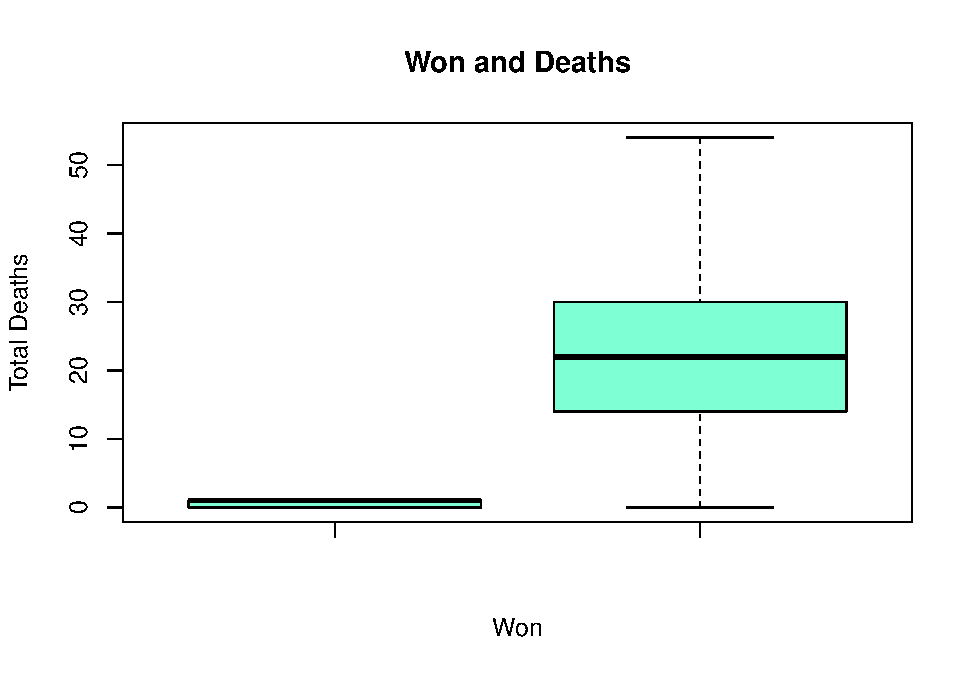
\includegraphics{Regression_files/figure-latex/unnamed-chunk-5-1.pdf}

\begin{Shaded}
\begin{Highlighting}[]
\FunctionTok{boxplot}\NormalTok{(full\_stats\_train}\SpecialCharTok{$}\NormalTok{won, full\_stats\_train}\SpecialCharTok{$}\NormalTok{TotalKill, }\AttributeTok{main=}\StringTok{"Won and kills"}\NormalTok{, }\AttributeTok{xlab=}\StringTok{"Won"}\NormalTok{, }\AttributeTok{ylab=}\StringTok{"Total kills"}\NormalTok{, }\AttributeTok{outline =} \ConstantTok{FALSE}\NormalTok{, }\AttributeTok{col =} \StringTok{\textquotesingle{}azure\textquotesingle{}}\NormalTok{)}
\end{Highlighting}
\end{Shaded}

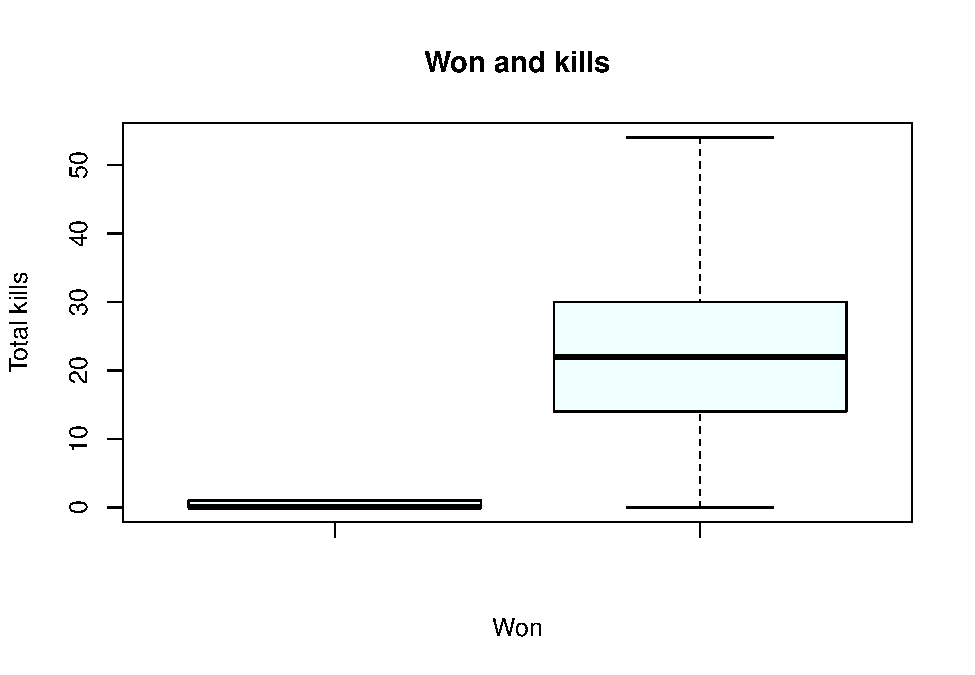
\includegraphics{Regression_files/figure-latex/unnamed-chunk-5-2.pdf}

\begin{Shaded}
\begin{Highlighting}[]
\FunctionTok{boxplot}\NormalTok{(full\_stats\_train}\SpecialCharTok{$}\NormalTok{won, full\_stats\_train}\SpecialCharTok{$}\NormalTok{TotalGold, }\AttributeTok{main=}\StringTok{"Won and Gold Earned"}\NormalTok{, }\AttributeTok{xlab=}\StringTok{"Won"}\NormalTok{, }\AttributeTok{ylab=}\StringTok{"Total Gold Earned"}\NormalTok{, }\AttributeTok{outline =} \ConstantTok{FALSE}\NormalTok{, }\AttributeTok{col =} \StringTok{\textquotesingle{}beige\textquotesingle{}}\NormalTok{)}
\end{Highlighting}
\end{Shaded}

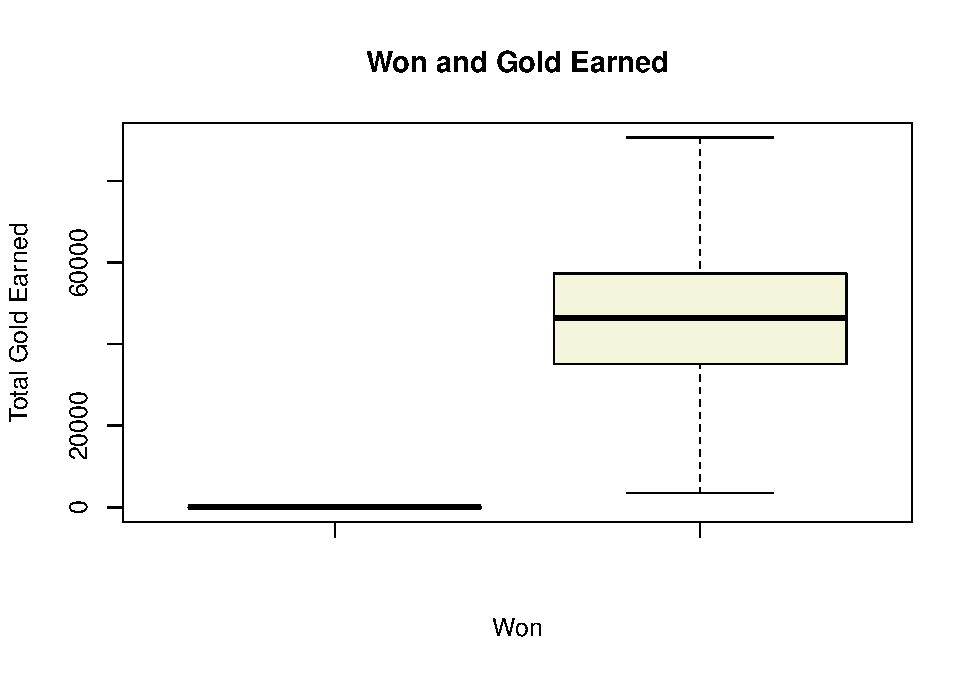
\includegraphics{Regression_files/figure-latex/unnamed-chunk-5-3.pdf}

\begin{Shaded}
\begin{Highlighting}[]
\FunctionTok{boxplot}\NormalTok{(full\_stats\_train}\SpecialCharTok{$}\NormalTok{won, full\_stats\_train}\SpecialCharTok{$}\NormalTok{TotalVision, }\AttributeTok{main=}\StringTok{"Won and Vision Score"}\NormalTok{, }\AttributeTok{xlab=}\StringTok{"Won"}\NormalTok{, }\AttributeTok{ylab=}\StringTok{"Total Vision Score"}\NormalTok{, }\AttributeTok{outline =} \ConstantTok{FALSE}\NormalTok{, }\AttributeTok{col =} \StringTok{\textquotesingle{}bisque\textquotesingle{}}\NormalTok{)}
\end{Highlighting}
\end{Shaded}

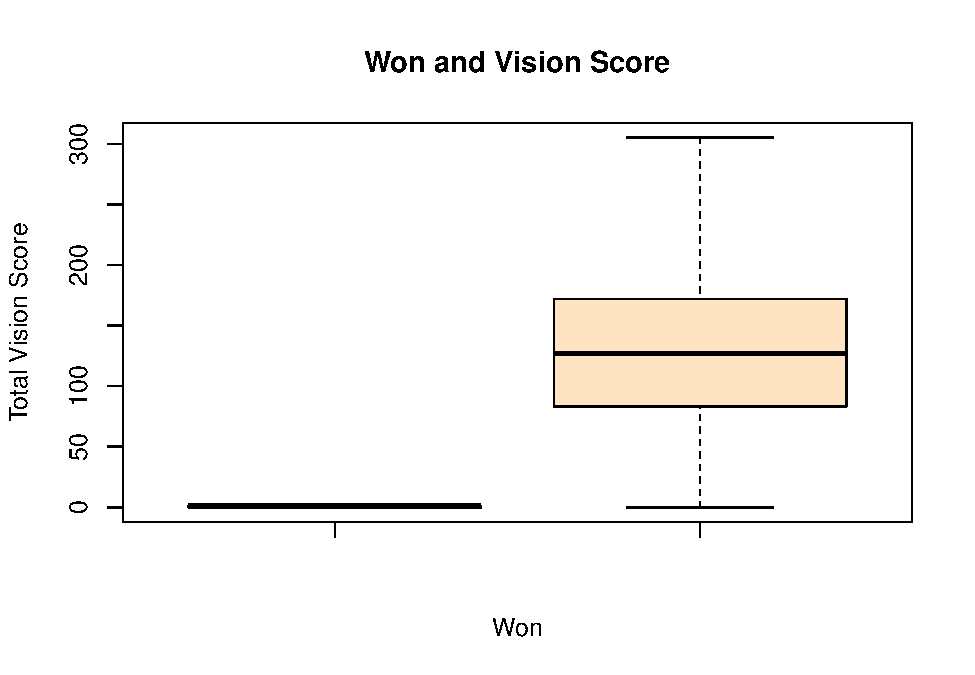
\includegraphics{Regression_files/figure-latex/unnamed-chunk-5-4.pdf}

\begin{Shaded}
\begin{Highlighting}[]
\FunctionTok{boxplot}\NormalTok{(full\_stats\_train}\SpecialCharTok{$}\NormalTok{won, full\_stats\_train}\SpecialCharTok{$}\NormalTok{TotalCrowdControl, }\AttributeTok{main=}\StringTok{"Won and totalTimeCrowdControlDealt"}\NormalTok{, }\AttributeTok{xlab=}\StringTok{"Won"}\NormalTok{, }\AttributeTok{ylab=}\StringTok{"Total totalTimeCrowdControlDealt"}\NormalTok{, }\AttributeTok{outline =} \ConstantTok{FALSE}\NormalTok{, }\AttributeTok{col=}\StringTok{\textquotesingle{}red\textquotesingle{}}\NormalTok{)}
\end{Highlighting}
\end{Shaded}

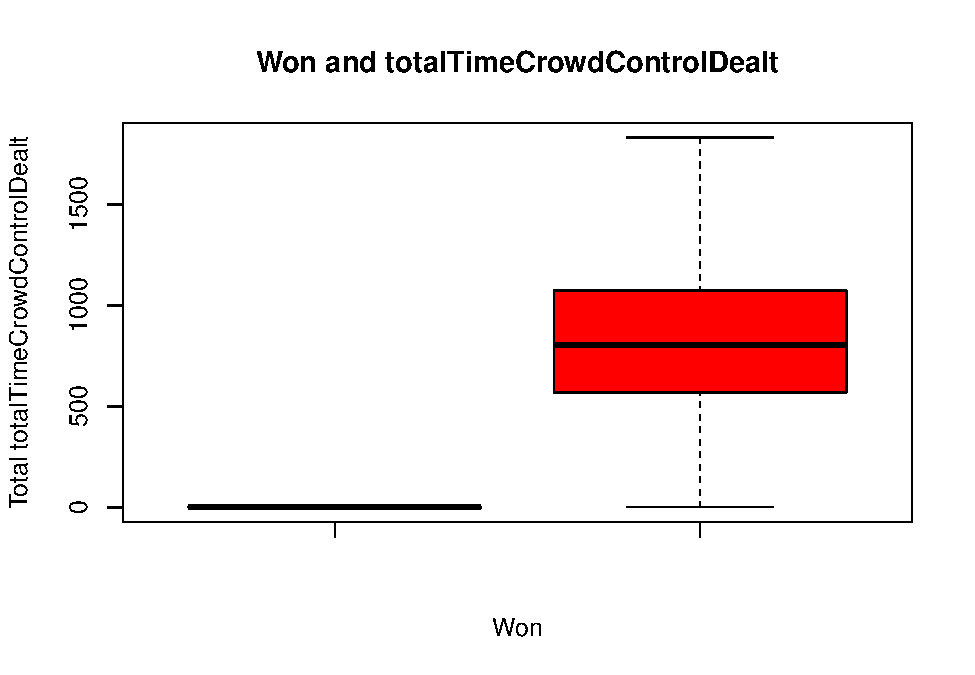
\includegraphics{Regression_files/figure-latex/unnamed-chunk-5-5.pdf}

\begin{Shaded}
\begin{Highlighting}[]
\FunctionTok{plot}\NormalTok{(full\_stats\_train}\SpecialCharTok{$}\NormalTok{TotalKill, full\_stats\_train}\SpecialCharTok{$}\NormalTok{TotalGold, }\AttributeTok{main=}\StringTok{"Kills and Gold Earned"}\NormalTok{, }\AttributeTok{xlab=}\StringTok{"Kills"}\NormalTok{, }\AttributeTok{ylab=}\StringTok{"Total Gold Earned"}\NormalTok{, }\AttributeTok{col =} \FunctionTok{rep}\NormalTok{(}\DecValTok{1}\SpecialCharTok{:}\DecValTok{6}\NormalTok{))}
\end{Highlighting}
\end{Shaded}

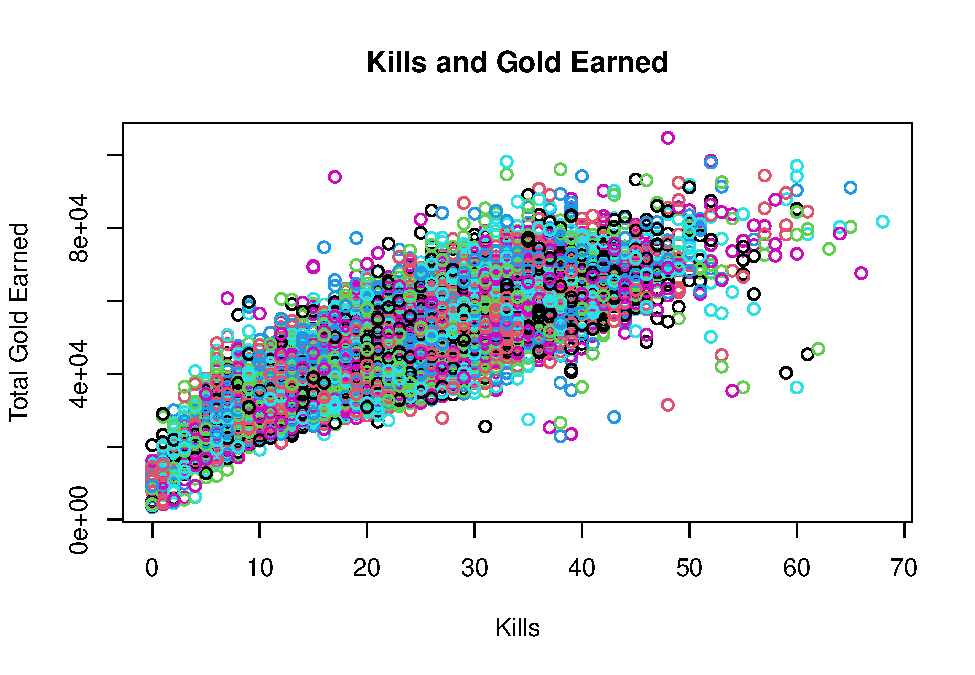
\includegraphics{Regression_files/figure-latex/unnamed-chunk-5-6.pdf}

\begin{Shaded}
\begin{Highlighting}[]
\FunctionTok{plot}\NormalTok{(full\_stats\_train}\SpecialCharTok{$}\NormalTok{TotalDeath, full\_stats\_train}\SpecialCharTok{$}\NormalTok{TotalDeath, }\AttributeTok{main=}\StringTok{"Deaths and Gold Earned"}\NormalTok{, }\AttributeTok{xlab=}\StringTok{"Deaths"}\NormalTok{, }\AttributeTok{ylab=}\StringTok{"Total Gold Earned"}\NormalTok{, }\AttributeTok{col =} \FunctionTok{rep}\NormalTok{(}\DecValTok{6}\SpecialCharTok{:}\DecValTok{12}\NormalTok{))}
\end{Highlighting}
\end{Shaded}

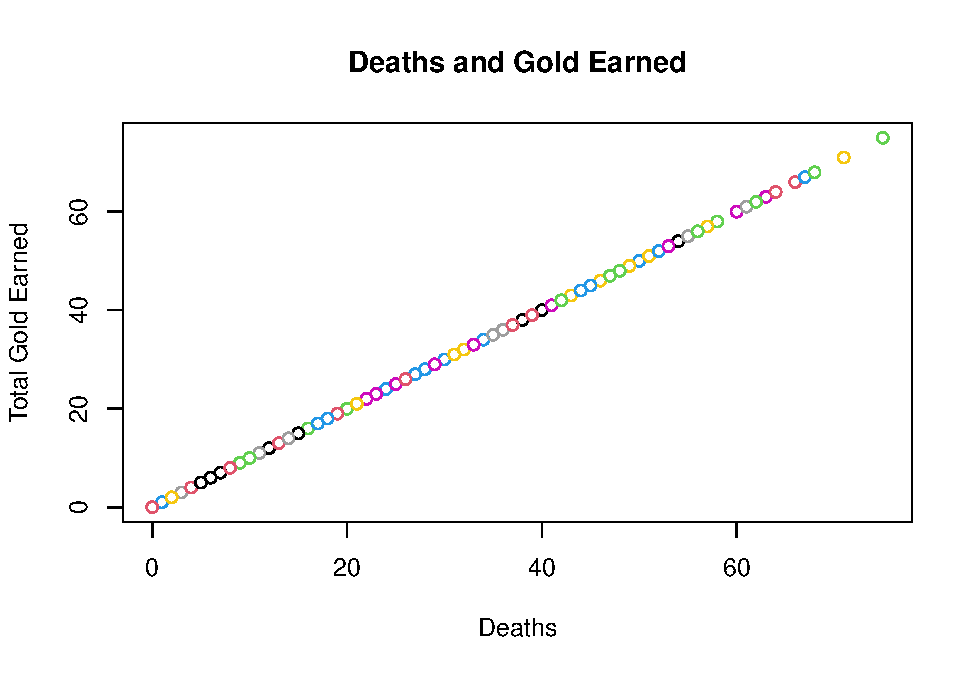
\includegraphics{Regression_files/figure-latex/unnamed-chunk-5-7.pdf}

\begin{Shaded}
\begin{Highlighting}[]
\FunctionTok{plot}\NormalTok{(full\_stats\_train}\SpecialCharTok{$}\NormalTok{TotalVision, full\_stats\_train}\SpecialCharTok{$}\NormalTok{TotalGold, }\AttributeTok{main=}\StringTok{"Vision Score and Gold Earned"}\NormalTok{, }\AttributeTok{xlab=}\StringTok{"Vision Score"}\NormalTok{, }\AttributeTok{ylab=}\StringTok{"Total Gold Earned"}\NormalTok{, }\AttributeTok{col =} \FunctionTok{rep}\NormalTok{(}\DecValTok{12}\SpecialCharTok{:}\DecValTok{18}\NormalTok{))}
\end{Highlighting}
\end{Shaded}

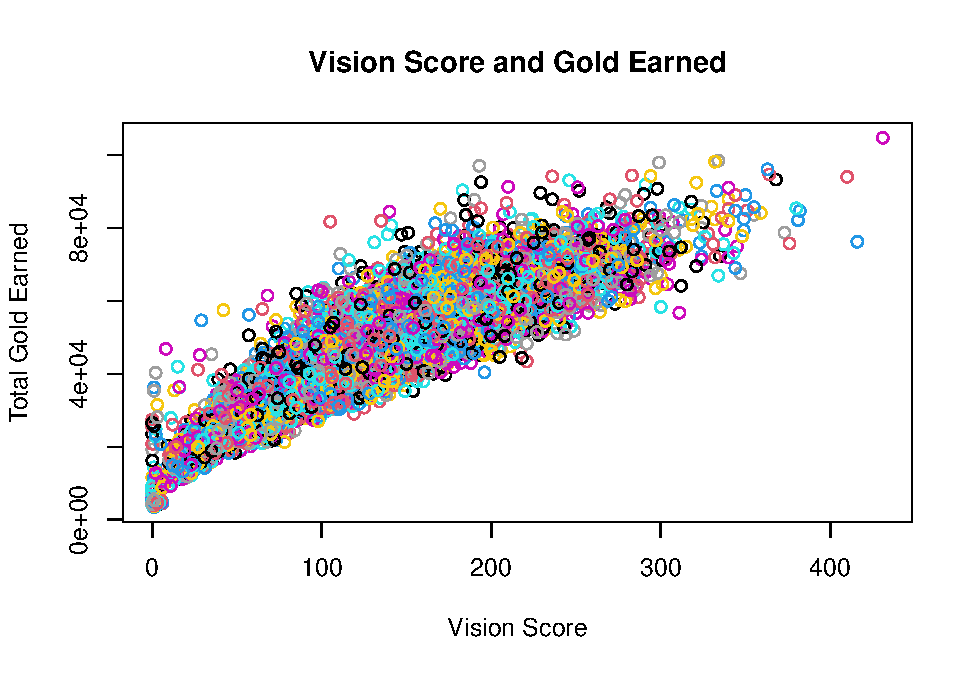
\includegraphics{Regression_files/figure-latex/unnamed-chunk-5-8.pdf}

\begin{Shaded}
\begin{Highlighting}[]
\FunctionTok{plot}\NormalTok{(full\_stats\_train}\SpecialCharTok{$}\NormalTok{TotalCrowdControl, full\_stats\_train}\SpecialCharTok{$}\NormalTok{TotalGold, }\AttributeTok{main=}\StringTok{"totalTimeCrowdControlDealt and Gold Earned"}\NormalTok{, }\AttributeTok{xlab=}\StringTok{"totalTimeCrowdControlDealt"}\NormalTok{, }\AttributeTok{ylab=}\StringTok{"Total Gold Earned"}\NormalTok{, }\AttributeTok{col =} \FunctionTok{rep}\NormalTok{(}\DecValTok{18}\SpecialCharTok{:}\DecValTok{24}\NormalTok{))}
\end{Highlighting}
\end{Shaded}

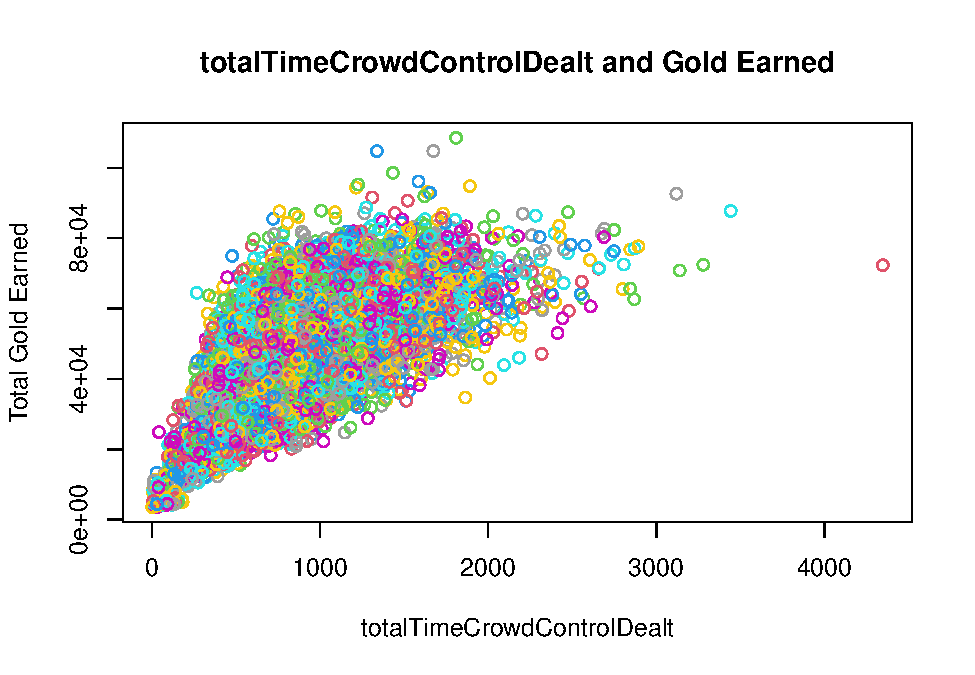
\includegraphics{Regression_files/figure-latex/unnamed-chunk-5-9.pdf}

\begin{Shaded}
\begin{Highlighting}[]
\FunctionTok{mean}\NormalTok{(full\_stats\_train}\SpecialCharTok{$}\NormalTok{TotalKill)}
\end{Highlighting}
\end{Shaded}

\begin{verbatim}
## [1] 22.51667
\end{verbatim}

\begin{Shaded}
\begin{Highlighting}[]
\FunctionTok{mean}\NormalTok{(full\_stats\_test}\SpecialCharTok{$}\NormalTok{TotalKill)}
\end{Highlighting}
\end{Shaded}

\begin{verbatim}
## [1] 22.80635
\end{verbatim}

\begin{Shaded}
\begin{Highlighting}[]
\FunctionTok{mean}\NormalTok{(full\_stats\_validate}\SpecialCharTok{$}\NormalTok{TotalKill)}
\end{Highlighting}
\end{Shaded}

\begin{verbatim}
## [1] 22.3826
\end{verbatim}

\hypertarget{svm-regression}{%
\subsection{SVM Regression}\label{svm-regression}}

\hypertarget{linear-regression}{%
\subsubsection{Linear Regression}\label{linear-regression}}

Trying linear regression with the data set

\begin{Shaded}
\begin{Highlighting}[]
\NormalTok{linreg }\OtherTok{\textless{}{-}} \FunctionTok{lm}\NormalTok{(won}\SpecialCharTok{\textasciitilde{}}\NormalTok{., }\AttributeTok{data=}\NormalTok{full\_stats\_train)}
\NormalTok{predLin }\OtherTok{\textless{}{-}} \FunctionTok{predict}\NormalTok{(linreg, }\AttributeTok{newdata=}\NormalTok{full\_stats\_test)}
\NormalTok{cor\_lin }\OtherTok{\textless{}{-}} \FunctionTok{cor}\NormalTok{(predLin, full\_stats\_test}\SpecialCharTok{$}\NormalTok{won)}
\NormalTok{mseLin }\OtherTok{\textless{}{-}} \FunctionTok{mean}\NormalTok{((predLin}\SpecialCharTok{{-}}\NormalTok{full\_stats\_test}\SpecialCharTok{$}\NormalTok{won)}\SpecialCharTok{\^{}}\DecValTok{2}\NormalTok{)}
\FunctionTok{summary}\NormalTok{(linreg)}
\end{Highlighting}
\end{Shaded}

\begin{verbatim}
## 
## Call:
## lm(formula = won ~ ., data = full_stats_train)
## 
## Residuals:
##      Min       1Q   Median       3Q      Max 
## -1.20718 -0.16501  0.00274  0.16277  1.70128 
## 
## Coefficients:
##                     Estimate Std. Error  t value Pr(>|t|)    
## (Intercept)        3.187e-01  1.167e-02   27.322  < 2e-16 ***
## TotalKill          2.201e-02  5.172e-04   42.567  < 2e-16 ***
## TotalDeath        -3.362e-02  2.985e-04 -112.649  < 2e-16 ***
## TotalDamage       -4.804e-07  2.475e-07   -1.941   0.0523 .  
## TotalGold          1.578e-05  6.911e-07   22.828  < 2e-16 ***
## TotalVision       -1.717e-03  9.917e-05  -17.314  < 2e-16 ***
## TotalCrowdControl -3.649e-05  8.446e-06   -4.320 1.57e-05 ***
## ---
## Signif. codes:  0 '***' 0.001 '**' 0.01 '*' 0.05 '.' 0.1 ' ' 1
## 
## Residual standard error: 0.2523 on 10853 degrees of freedom
## Multiple R-squared:  0.7456, Adjusted R-squared:  0.7455 
## F-statistic:  5302 on 6 and 10853 DF,  p-value: < 2.2e-16
\end{verbatim}

\hypertarget{training}{%
\paragraph{Training}\label{training}}

Now we will build our SVM Linear model

\begin{Shaded}
\begin{Highlighting}[]
\FunctionTok{library}\NormalTok{(e1071)}
\NormalTok{svm\_won }\OtherTok{\textless{}{-}} \FunctionTok{svm}\NormalTok{(won}\SpecialCharTok{\textasciitilde{}}\NormalTok{., }\AttributeTok{data=}\NormalTok{full\_stats\_train, }\AttributeTok{kernel=}\StringTok{"linear"}\NormalTok{, }\AttributeTok{cost=}\DecValTok{10}\NormalTok{, }\AttributeTok{scale=}\ConstantTok{TRUE}\NormalTok{)}
\FunctionTok{summary}\NormalTok{(svm\_won)}
\end{Highlighting}
\end{Shaded}

\begin{verbatim}
## 
## Call:
## svm(formula = won ~ ., data = full_stats_train, kernel = "linear", 
##     cost = 10, scale = TRUE)
## 
## 
## Parameters:
##    SVM-Type:  eps-regression 
##  SVM-Kernel:  linear 
##        cost:  10 
##       gamma:  0.1666667 
##     epsilon:  0.1 
## 
## 
## Number of Support Vectors:  9045
\end{verbatim}

\hypertarget{testing-evaluation}{%
\paragraph{Testing \& Evaluation}\label{testing-evaluation}}

Now we can evaluate on the test set:

\begin{Shaded}
\begin{Highlighting}[]
\FunctionTok{library}\NormalTok{(caret)}
\end{Highlighting}
\end{Shaded}

\begin{verbatim}
## Loading required package: ggplot2
\end{verbatim}

\begin{verbatim}
## Loading required package: lattice
\end{verbatim}

\begin{Shaded}
\begin{Highlighting}[]
\NormalTok{svm\_probs }\OtherTok{\textless{}{-}} \FunctionTok{predict}\NormalTok{(svm\_won, }\AttributeTok{newdata =}\NormalTok{ full\_stats\_test)}
\NormalTok{svm\_pred }\OtherTok{\textless{}{-}} \FunctionTok{ifelse}\NormalTok{(svm\_probs }\SpecialCharTok{\textgreater{}} \FloatTok{0.5}\NormalTok{, }\DecValTok{1}\NormalTok{, }\DecValTok{0}\NormalTok{)}
\NormalTok{svm\_acc }\OtherTok{\textless{}{-}} \FunctionTok{mean}\NormalTok{(svm\_pred }\SpecialCharTok{==}\NormalTok{ full\_stats\_test}\SpecialCharTok{$}\NormalTok{won)}

\FunctionTok{confusionMatrix}\NormalTok{(}\FunctionTok{as.factor}\NormalTok{(svm\_pred), }\AttributeTok{reference =} \FunctionTok{as.factor}\NormalTok{(full\_stats\_test}\SpecialCharTok{$}\NormalTok{won))}
\end{Highlighting}
\end{Shaded}

\begin{verbatim}
## Confusion Matrix and Statistics
## 
##           Reference
## Prediction    0    1
##          0 1714   62
##          1   77 1767
##                                           
##                Accuracy : 0.9616          
##                  95% CI : (0.9548, 0.9676)
##     No Information Rate : 0.5052          
##     P-Value [Acc > NIR] : <2e-16          
##                                           
##                   Kappa : 0.9232          
##                                           
##  Mcnemar's Test P-Value : 0.235           
##                                           
##             Sensitivity : 0.9570          
##             Specificity : 0.9661          
##          Pos Pred Value : 0.9651          
##          Neg Pred Value : 0.9582          
##              Prevalence : 0.4948          
##          Detection Rate : 0.4735          
##    Detection Prevalence : 0.4906          
##       Balanced Accuracy : 0.9616          
##                                           
##        'Positive' Class : 0               
## 
\end{verbatim}

\hypertarget{tuning}{%
\paragraph{Tuning}\label{tuning}}

\begin{Shaded}
\begin{Highlighting}[]
\NormalTok{predLinSvm }\OtherTok{\textless{}{-}} \FunctionTok{predict}\NormalTok{(svm\_won, }\AttributeTok{newdata=}\NormalTok{full\_stats\_test)}
\NormalTok{corLinSvm }\OtherTok{\textless{}{-}} \FunctionTok{cor}\NormalTok{(predLinSvm, full\_stats\_test}\SpecialCharTok{$}\NormalTok{won)}
\NormalTok{mseLinSvm }\OtherTok{\textless{}{-}} \FunctionTok{mean}\NormalTok{((predLinSvm }\SpecialCharTok{{-}}\NormalTok{ full\_stats\_test}\SpecialCharTok{$}\NormalTok{won)}\SpecialCharTok{\^{}}\DecValTok{2}\NormalTok{)}

\NormalTok{tuneLin }\OtherTok{\textless{}{-}} \FunctionTok{tune}\NormalTok{(svm, won}\SpecialCharTok{\textasciitilde{}}\NormalTok{., }\AttributeTok{data=}\NormalTok{full\_stats\_validate, }\AttributeTok{kernel=}\StringTok{"linear"}\NormalTok{, }\AttributeTok{ranges=}\FunctionTok{list}\NormalTok{(}\AttributeTok{cost=}\FunctionTok{c}\NormalTok{(}\FloatTok{0.001}\NormalTok{, }\FloatTok{0.01}\NormalTok{, }\FloatTok{0.1}\NormalTok{, }\DecValTok{1}\NormalTok{, }\DecValTok{5}\NormalTok{, }\DecValTok{10}\NormalTok{, }\DecValTok{100}\NormalTok{)))}
\FunctionTok{summary}\NormalTok{(tuneLin)}
\end{Highlighting}
\end{Shaded}

\begin{verbatim}
## 
## Parameter tuning of 'svm':
## 
## - sampling method: 10-fold cross validation 
## 
## - best parameters:
##  cost
##  0.01
## 
## - best performance: 0.0684552 
## 
## - Detailed performance results:
##    cost      error  dispersion
## 1 1e-03 0.07378850 0.005199356
## 2 1e-02 0.06845520 0.005147546
## 3 1e-01 0.06863610 0.005162625
## 4 1e+00 0.06868263 0.005171140
## 5 5e+00 0.06868545 0.005163666
## 6 1e+01 0.06868161 0.005164354
## 7 1e+02 0.06867464 0.005176276
\end{verbatim}

\hypertarget{polynomial-kernel}{%
\paragraph{Polynomial Kernel}\label{polynomial-kernel}}

\begin{Shaded}
\begin{Highlighting}[]
\NormalTok{svm\_poly }\OtherTok{\textless{}{-}} \FunctionTok{svm}\NormalTok{(won}\SpecialCharTok{\textasciitilde{}}\NormalTok{., }\AttributeTok{data=}\NormalTok{full\_stats\_train, }\AttributeTok{kernel=}\StringTok{"polynomial"}\NormalTok{, }\AttributeTok{cost=}\DecValTok{10}\NormalTok{, }\AttributeTok{scale=}\ConstantTok{TRUE}\NormalTok{)}
\FunctionTok{summary}\NormalTok{(svm\_poly)}
\end{Highlighting}
\end{Shaded}

\begin{verbatim}
## 
## Call:
## svm(formula = won ~ ., data = full_stats_train, kernel = "polynomial", 
##     cost = 10, scale = TRUE)
## 
## 
## Parameters:
##    SVM-Type:  eps-regression 
##  SVM-Kernel:  polynomial 
##        cost:  10 
##      degree:  3 
##       gamma:  0.1666667 
##      coef.0:  0 
##     epsilon:  0.1 
## 
## 
## Number of Support Vectors:  10033
\end{verbatim}

\hypertarget{testing-evaluation-1}{%
\paragraph{Testing \& Evaluation}\label{testing-evaluation-1}}

Now we can evaluate on the test set:

\begin{Shaded}
\begin{Highlighting}[]
\NormalTok{predPolySvm }\OtherTok{\textless{}{-}} \FunctionTok{predict}\NormalTok{(svm\_poly, }\AttributeTok{newdata=}\NormalTok{full\_stats\_test)}
\NormalTok{corPolySvm }\OtherTok{\textless{}{-}} \FunctionTok{cor}\NormalTok{(predPolySvm, full\_stats\_test}\SpecialCharTok{$}\NormalTok{won)}
\NormalTok{svm\_poly }\OtherTok{\textless{}{-}} \FunctionTok{ifelse}\NormalTok{(predPolySvm }\SpecialCharTok{\textgreater{}} \FloatTok{0.5}\NormalTok{, }\DecValTok{1}\NormalTok{, }\DecValTok{0}\NormalTok{)}
\NormalTok{msePolySvm }\OtherTok{\textless{}{-}} \FunctionTok{mean}\NormalTok{((predPolySvm }\SpecialCharTok{{-}}\NormalTok{ full\_stats\_test}\SpecialCharTok{$}\NormalTok{won)}\SpecialCharTok{\^{}}\DecValTok{2}\NormalTok{)}

\FunctionTok{confusionMatrix}\NormalTok{(}\FunctionTok{as.factor}\NormalTok{(svm\_poly), }\AttributeTok{reference =} \FunctionTok{as.factor}\NormalTok{(full\_stats\_test}\SpecialCharTok{$}\NormalTok{won))}
\end{Highlighting}
\end{Shaded}

\begin{verbatim}
## Confusion Matrix and Statistics
## 
##           Reference
## Prediction    0    1
##          0 1651   55
##          1  140 1774
##                                           
##                Accuracy : 0.9461          
##                  95% CI : (0.9383, 0.9533)
##     No Information Rate : 0.5052          
##     P-Value [Acc > NIR] : < 2.2e-16       
##                                           
##                   Kappa : 0.8922          
##                                           
##  Mcnemar's Test P-Value : 1.795e-09       
##                                           
##             Sensitivity : 0.9218          
##             Specificity : 0.9699          
##          Pos Pred Value : 0.9678          
##          Neg Pred Value : 0.9269          
##              Prevalence : 0.4948          
##          Detection Rate : 0.4561          
##    Detection Prevalence : 0.4713          
##       Balanced Accuracy : 0.9459          
##                                           
##        'Positive' Class : 0               
## 
\end{verbatim}

\hypertarget{radial-kernel}{%
\paragraph{Radial Kernel}\label{radial-kernel}}

\begin{Shaded}
\begin{Highlighting}[]
\NormalTok{svm\_rad }\OtherTok{\textless{}{-}} \FunctionTok{svm}\NormalTok{(won}\SpecialCharTok{\textasciitilde{}}\NormalTok{., }\AttributeTok{data=}\NormalTok{full\_stats\_train, }\AttributeTok{kernel=}\StringTok{"radial"}\NormalTok{, }\AttributeTok{cost=}\DecValTok{10}\NormalTok{, }\AttributeTok{scale=}\ConstantTok{TRUE}\NormalTok{)}
\FunctionTok{summary}\NormalTok{(svm\_rad)}
\end{Highlighting}
\end{Shaded}

\begin{verbatim}
## 
## Call:
## svm(formula = won ~ ., data = full_stats_train, kernel = "radial", 
##     cost = 10, scale = TRUE)
## 
## 
## Parameters:
##    SVM-Type:  eps-regression 
##  SVM-Kernel:  radial 
##        cost:  10 
##       gamma:  0.1666667 
##     epsilon:  0.1 
## 
## 
## Number of Support Vectors:  4956
\end{verbatim}

\hypertarget{testing-evaluation-2}{%
\paragraph{Testing \& Evaluation}\label{testing-evaluation-2}}

Now we can evaluate on the test set:

\begin{Shaded}
\begin{Highlighting}[]
\NormalTok{predRadSvm }\OtherTok{\textless{}{-}} \FunctionTok{predict}\NormalTok{(svm\_rad, }\AttributeTok{newdata=}\NormalTok{full\_stats\_test)}
\NormalTok{corRadSvm }\OtherTok{\textless{}{-}} \FunctionTok{cor}\NormalTok{(predRadSvm, full\_stats\_test}\SpecialCharTok{$}\NormalTok{won)}
\NormalTok{mseRadSvm }\OtherTok{\textless{}{-}} \FunctionTok{mean}\NormalTok{((predRadSvm }\SpecialCharTok{{-}}\NormalTok{ full\_stats\_test}\SpecialCharTok{$}\NormalTok{won)}\SpecialCharTok{\^{}}\DecValTok{2}\NormalTok{)}
\NormalTok{svm\_rad }\OtherTok{\textless{}{-}} \FunctionTok{ifelse}\NormalTok{(predRadSvm }\SpecialCharTok{\textgreater{}} \FloatTok{0.5}\NormalTok{, }\DecValTok{1}\NormalTok{, }\DecValTok{0}\NormalTok{)}

\FunctionTok{confusionMatrix}\NormalTok{(}\FunctionTok{as.factor}\NormalTok{(svm\_poly), }\AttributeTok{reference =} \FunctionTok{as.factor}\NormalTok{(full\_stats\_test}\SpecialCharTok{$}\NormalTok{won))}
\end{Highlighting}
\end{Shaded}

\begin{verbatim}
## Confusion Matrix and Statistics
## 
##           Reference
## Prediction    0    1
##          0 1651   55
##          1  140 1774
##                                           
##                Accuracy : 0.9461          
##                  95% CI : (0.9383, 0.9533)
##     No Information Rate : 0.5052          
##     P-Value [Acc > NIR] : < 2.2e-16       
##                                           
##                   Kappa : 0.8922          
##                                           
##  Mcnemar's Test P-Value : 1.795e-09       
##                                           
##             Sensitivity : 0.9218          
##             Specificity : 0.9699          
##          Pos Pred Value : 0.9678          
##          Neg Pred Value : 0.9269          
##              Prevalence : 0.4948          
##          Detection Rate : 0.4561          
##    Detection Prevalence : 0.4713          
##       Balanced Accuracy : 0.9459          
##                                           
##        'Positive' Class : 0               
## 
\end{verbatim}

\hypertarget{tune-hyperparameters}{%
\paragraph{Tune Hyperparameters}\label{tune-hyperparameters}}

\begin{Shaded}
\begin{Highlighting}[]
\FunctionTok{set.seed}\NormalTok{(}\DecValTok{1234}\NormalTok{)}

\NormalTok{tuneRad }\OtherTok{\textless{}{-}} \FunctionTok{tune}\NormalTok{(svm, won}\SpecialCharTok{\textasciitilde{}}\NormalTok{., }\AttributeTok{data=}\NormalTok{full\_stats\_validate, }\AttributeTok{kernel=}\StringTok{"radial"}\NormalTok{, }\AttributeTok{ranges=}\FunctionTok{list}\NormalTok{(}\AttributeTok{cost=}\FunctionTok{c}\NormalTok{(}\FloatTok{0.1}\NormalTok{,}\DecValTok{1}\NormalTok{,}\DecValTok{10}\NormalTok{,}\DecValTok{100}\NormalTok{,}\DecValTok{1000}\NormalTok{), }\AttributeTok{gamma=}\FunctionTok{c}\NormalTok{(}\FloatTok{0.5}\NormalTok{,}\DecValTok{1}\NormalTok{,}\DecValTok{2}\NormalTok{,}\DecValTok{3}\NormalTok{,}\DecValTok{4}\NormalTok{)))}
\FunctionTok{summary}\NormalTok{(tuneRad)}
\end{Highlighting}
\end{Shaded}

\begin{verbatim}
## 
## Parameter tuning of 'svm':
## 
## - sampling method: 10-fold cross validation 
## 
## - best parameters:
##  cost gamma
##     1   0.5
## 
## - best performance: 0.04325315 
## 
## - Detailed performance results:
##     cost gamma      error  dispersion
## 1  1e-01   0.5 0.04638689 0.004707507
## 2  1e+00   0.5 0.04325315 0.005309547
## 3  1e+01   0.5 0.04876789 0.004557089
## 4  1e+02   0.5 0.06733271 0.007390659
## 5  1e+03   0.5 0.14129115 0.020743389
## 6  1e-01   1.0 0.04803253 0.004444556
## 7  1e+00   1.0 0.04502955 0.005546540
## 8  1e+01   1.0 0.05228316 0.006012679
## 9  1e+02   1.0 0.07954230 0.008617296
## 10 1e+03   1.0 0.16524801 0.019899388
## 11 1e-01   2.0 0.05771367 0.003501254
## 12 1e+00   2.0 0.04837947 0.005679430
## 13 1e+01   2.0 0.06071113 0.007527551
## 14 1e+02   2.0 0.08448434 0.010883670
## 15 1e+03   2.0 0.08939843 0.011644936
## 16 1e-01   3.0 0.06988417 0.003350043
## 17 1e+00   3.0 0.05425049 0.005472039
## 18 1e+01   3.0 0.06546445 0.007576974
## 19 1e+02   3.0 0.07070319 0.008125758
## 20 1e+03   3.0 0.07250023 0.008463633
## 21 1e-01   4.0 0.08373831 0.003355149
## 22 1e+00   4.0 0.06082808 0.005298901
## 23 1e+01   4.0 0.06884024 0.007211495
## 24 1e+02   4.0 0.06932821 0.006886294
## 25 1e+03   4.0 0.07144663 0.006893228
\end{verbatim}

\begin{Shaded}
\begin{Highlighting}[]
\NormalTok{svm\_radTune }\OtherTok{\textless{}{-}} \FunctionTok{svm}\NormalTok{(won}\SpecialCharTok{\textasciitilde{}}\NormalTok{., }\AttributeTok{data=}\NormalTok{full\_stats\_validate, }\AttributeTok{kernel=}\StringTok{"radial"}\NormalTok{, }\AttributeTok{cost=}\DecValTok{100}\NormalTok{, }\AttributeTok{gamma=}\FloatTok{0.5}\NormalTok{, }\AttributeTok{scale=}\ConstantTok{TRUE}\NormalTok{)}
\FunctionTok{summary}\NormalTok{(svm\_radTune)}
\end{Highlighting}
\end{Shaded}

\begin{verbatim}
## 
## Call:
## svm(formula = won ~ ., data = full_stats_validate, kernel = "radial", 
##     cost = 100, gamma = 0.5, scale = TRUE)
## 
## 
## Parameters:
##    SVM-Type:  eps-regression 
##  SVM-Kernel:  radial 
##        cost:  100 
##       gamma:  0.5 
##     epsilon:  0.1 
## 
## 
## Number of Support Vectors:  1780
\end{verbatim}

\begin{Shaded}
\begin{Highlighting}[]
\NormalTok{predRadSvm1 }\OtherTok{\textless{}{-}} \FunctionTok{predict}\NormalTok{(svm\_radTune, }\AttributeTok{newdata=}\NormalTok{full\_stats\_test)}
\NormalTok{corRadSvm1 }\OtherTok{\textless{}{-}} \FunctionTok{cor}\NormalTok{(predRadSvm1, full\_stats\_test}\SpecialCharTok{$}\NormalTok{won)}
\NormalTok{mseRadSvm1 }\OtherTok{\textless{}{-}} \FunctionTok{mean}\NormalTok{((predRadSvm1 }\SpecialCharTok{{-}}\NormalTok{ full\_stats\_test}\SpecialCharTok{$}\NormalTok{won)}\SpecialCharTok{\^{}}\DecValTok{2}\NormalTok{)}
\end{Highlighting}
\end{Shaded}

\hypertarget{svm-linear-vs-polynomial-vs-radial-kernels}{%
\subsection{SVM Linear vs Polynomial vs Radial
Kernels}\label{svm-linear-vs-polynomial-vs-radial-kernels}}

Analyzing the results of each model based on the algorithms.

\hypertarget{svm-linear}{%
\subsubsection{SVM Linear}\label{svm-linear}}

For this we are trying to predict whether or not a team has won a match
using the stats they had at the end of a game. Linear SVM works by
plotting the data in a high-dimensional feature space so that the points
can be categorized. The data is then transformed in ways that allows a
separator to be drawn as a hyper plane. Linear kernels are better for
when the data can be linearly separated easily.

For this data set there was little difference between the accuracies in
the different kernel types, which may mean this data was easy to split
regardless of the kernel type. The linear kernel did perform marginally
better than the others.

\hypertarget{svm-polynomial}{%
\subsubsection{SVM Polynomial}\label{svm-polynomial}}

Polynomial kernels behave similarly to the linear kernels. However, they
put all the data in a feature space over polynomials of the original
variables, meaning that they work better for data that isn't easily
separated linearly.

This performed slightly worse than linear kernel, meaning this dataset
was easily split using a linear hyperplane. However, it was still very
accurate. \#\#\# SVM Radial Kernels

Radial kernels are similar to polynomial kernels as they both work with
data that cannot be linearly separated easily. This generates a
non-linear decision boundary.

This performed slightly worse than linear kernel, meaning this dataset
was easily split using a linear hyperplane. However, it was still very
accurate.

\end{document}
